\documentclass[12pt,a4paper, oneside]{article}
\usepackage[utf8]{inputenc}
\usepackage[T1]{fontenc}
\usepackage[english,german]{babel}
\usepackage[style=german]{csquotes}
\usepackage{graphicx}

\author{Uni Oldenburg, SWP2020 Gruppe A}

\begin{document}

    \begin{titlepage}
        \pagestyle{empty}
        \begin{center}

            \begin{figure}[h]
                \centering
                
\includegraphics[width=0.35\textwidth]{../img/Logo.jpg}
            \end{figure}

            \bigskip \bigskip \noindent
            \textsc{\textbf{\LARGE Softwareprojekt:}} \par \bigskip \noindent
            \textsc{\textbf{\LARGE Projekttagebuch}}


            \par \bigskip \bigskip \bigskip \bigskip \bigskip \noindent
            {\Large Gruppe A} \par \medskip \noindent

            \par \bigskip \bigskip \bigskip \bigskip \bigskip \bigskip \noindent
            \textit{\Large Wintersemester 2020/21 und} \par \noindent
            \textit{\Large Sommersemester 2021}

            \par \bigskip \bigskip \bigskip \bigskip \bigskip \bigskip \noindent
            \par \bigskip \bigskip \bigskip \noindent
            {\Large Sprintanalyse} \par \medskip \noindent

        \end{center}
    \end{titlepage}

    \tableofcontents
    \pagebreak


    \section{Sprinttagebuch: Sprint-Nr. 2}
    \underline{Name des Sprints:}
    \\
    Sprint 2: Electric Boogaloo

    \noindent
    \\
    \underline{Zeitraum des Sprints:}
    \\
    10. Dezember 2020 - 22. Dezember 2020

    \noindent
    \\
    \underline{Ziel des Sprints:}
    \\
    Funktionales Hauptmenü, grundlegende Lobbyfunktionalitäten und ein Chat

    \noindent
    \\
    \underline {Team:}
    \\
    Sven Ahrens, Alwin Bossert, Aldin Dervisi, Marvin Drees, Mario Fokken,
    Timo Gerken, Finn Haase, Temmo Junkhoff, Maximilian Lindner, Steven Luong, Phillip-André Suhr, Eric Vuong


    \section{Vorgänge}

    \begin{itemize}

        \item SWP2020A-32: Als Nutzer möchte ich beim Erstellen einer Lobby die Lobby frei benennen, damit Freunde einfacher der Lobby beitreten können. (7 Story Points)

        \item SWP2020A-47: Als Nutzer möchte ich vom Hauptmenü einer der dort sichtbaren Lobbys beitreten können. (3 Story Points)

        \item SWP2020A-48: Als Nutzer möchte ich die existierenden Lobbys im Hauptmenü sehen können. (7 Story Points)

        \item SWP2020A-49: Als Nutzer möchte ich mit einem Button im Hauptmenü mein Passwort ändern können. (8 Story Points)

        \item SWP2020A-50: ANmi vom Fenster einer Lobby aus diese verlassen können. (7 Story Points)

        \item SWP2020A-51: Als Nutzer möchte ich im Fenster einer Lobby sehen können, welche Spieler sich aktuell in ihr befinden. (5 Story Points)

        \item SWP2020A-52: Als Nutzer möchte ich eine Chatansicht sehen können. (6 Story Points)

        \item SWP2020A-53: ANmi immer die neuesten Nachrichten im Chat sehen können, damit ich der aktuellen Unterhaltung folgen kann (14 Story Points)

        \item (\textit{Nachgezogen}) SWP2020A-73: UserDeletionRequest wird nicht fertig abgehandelt (2 Story Points)
    \end{itemize}

    \subsection{Sprinterfolg}
    \begin{figure}[h]
        \centering
        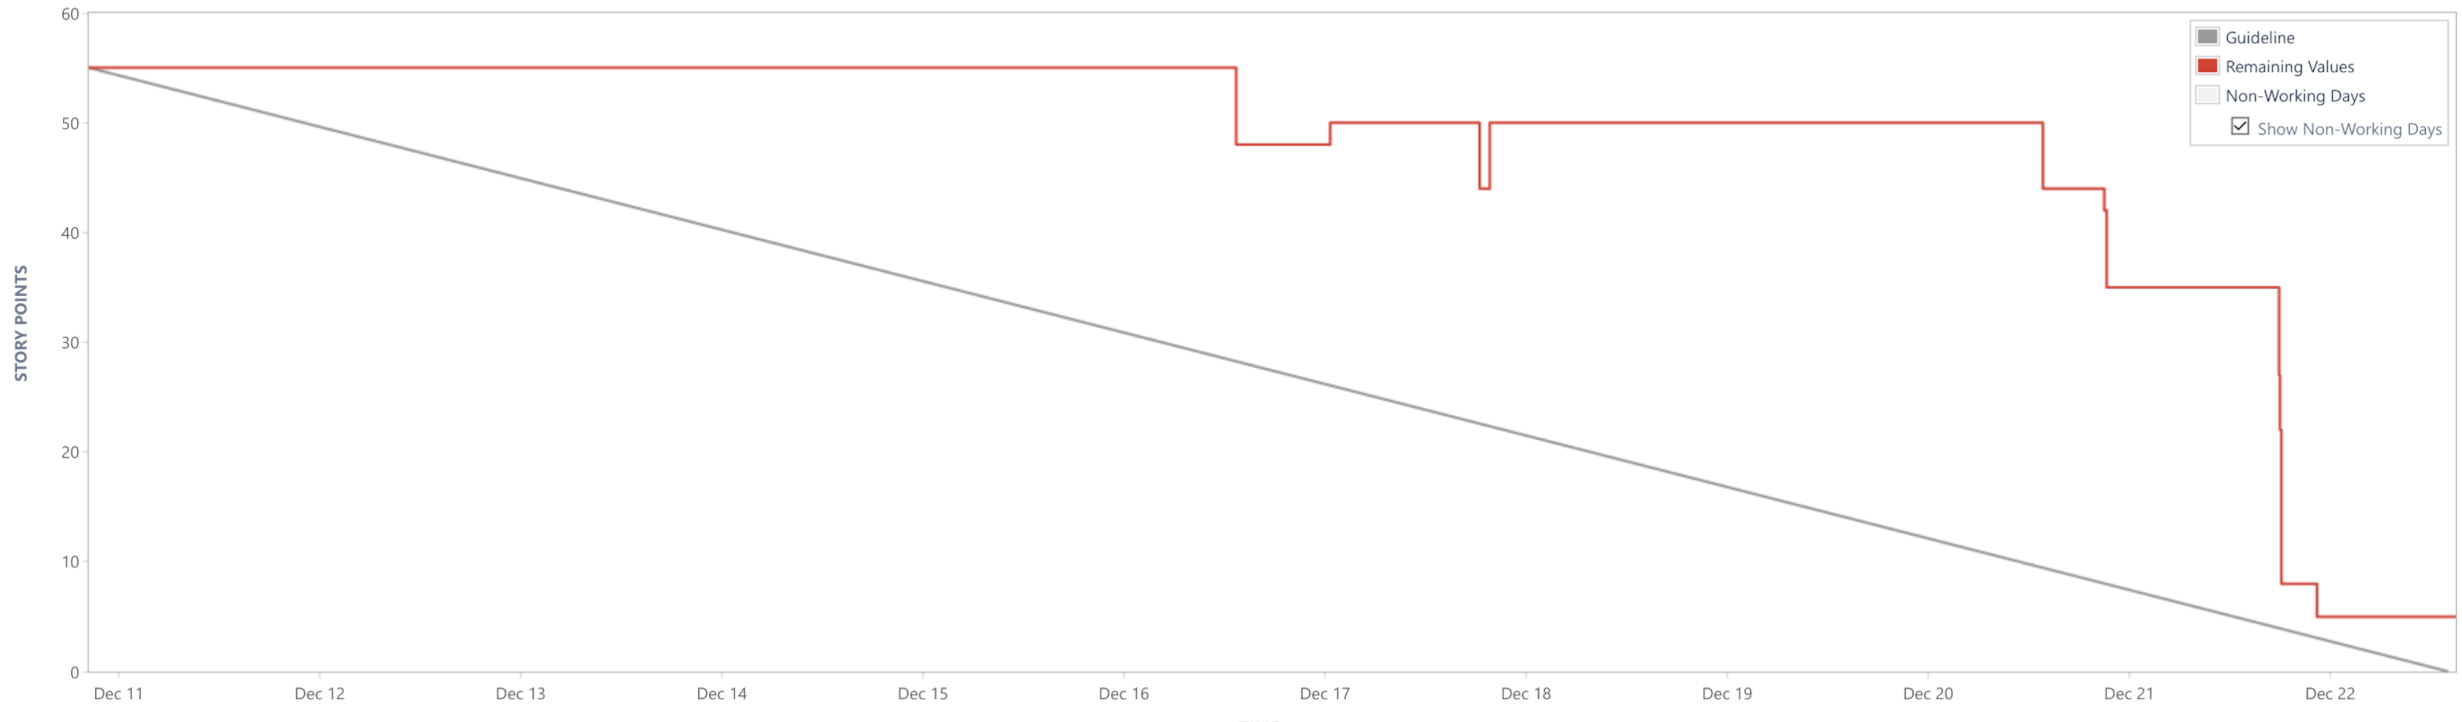
\includegraphics[width=\textwidth, height=5cm]{../img/sprint_02/Burndown-Sprint2.PNG}
        \caption{Burndown-Diagramm Sprint 2}
        \label{fig: Burndown-Sprint2}
    \end{figure}

    \noindent
    Zum Startpunkt des Sprints belief sich der Aufwand des Sprints auf 8 Vorgänge mit insgesamt 55 Story Points. Am 17. Dezember 2020 wurde dann der Vorgang \textit{SWP2020A-73: UserDeletionRequest wird nicht fertig abgehandelt (Bugfix)} (2 Story Points) nachgezogen, womit sich der Gesamtaufwand des Sprints auf 9 Vorgänge mit insgesamt 57 Story Points erhöht hat. Wenn man das Burndown Diagramm dieses Sprints mit dem des Vorherigen vergleicht wir deutlich, dass sich unsere Velocity deutlich gesteigert hat. Das, aus der Retrospektive von Sprint 1, gewonnene Wissen konnte durchaus umgesetzt werden, sodass die meisten Vorgänge bis Sprintende erfolgreich beendet wurden. Lediglich der mit 5 Story Points geschätzte Vorgang \textit{SWP2020A-50: ANmi vom Fenster einer Lobby aus diese verlassen können.} konnte nicht bis zum Sprintende am 22. Dezember 2020 beendet werden. Bis zu diesem Zeitpunkt wurden 8 Vorgänge mit insgesamt 50 Story Points fertig bearbeitet.

    \subsection{Sprintprobleme bzw. Hindernisse}

    Im Gegensatz zum 1. Sprint wurden Deadlines zum größten Teil durchgängig eingehalten. Das folgt zum Einen daraus, dass ein, für alle Teammitglieder verständlicher, Commit- und Reviewfreeze eingeführt und auch so kommuniziert wurde. Zum Anderen wurde aus der vorangegangenen Retrospektive von Sprint 1 mitgenommen, dass die Bearbeitung der Vorgänge deutlich früher begonnen werden muss. Das diese Erkenntnis aber so wage festgehalten wurde wie im vorherigen Satz beschrieben führte dazu, dass die Bearbeitung der Vorgänge zwar früher begann aber die Aufgaben allgemein sehr spät im Sprint beendet wurden. Diese Tatsache geht auch aus dem Burndown Diagramm deutlich hervor.


    \section{Erkenntnis aus der Retrospektive}

    Folgende Erkenntnisse ergaben sich aus der Retrospektive:\\

    \underline{Was lief gut?}
    \begin{itemize}
        \item Pairprogramming beibehalten
        \item Aktuelle Kommunikation beibehalten
        \\
    \end{itemize}

    \underline{Was lief nicht so gut?}
    \begin{itemize}
        \item Reviews möglichst früh durchführen
        \item Aktuelles Zeitmanagement optimieren
        \item Auf Review-bereite PR hinweisen bspw. auf Discord
        \item Aufgaben schon in der ersten Woche grundlegend abarbeiten
        \\
    \end{itemize}

    \underline{Was sollte anders laufen?}
    \begin{itemize}
        \item Abhängigkeiten möglichst vermeiden
        \item Bei unausweichlichen Abhängigkeiten frühere Deadline für die blockierenden Storys
        \item Öfter den develop-Branch in den Story-Branch mergen um (große) Konflikte zu verhindern
        \item Auf Englisch (UK) vereinheitlichen
        \item Pair-Programming-Partner tauschen
    \end{itemize}


    \section{Sonstige Anmerkungen}
    Das Einführen der klar verständlichen Commit- und Reviewfreezes hat dazu geführt, dass mögliche Missverständnisse aus dem Weg geräumt wurden, bevor diese hätten aufkommen können. Ebenso hat sich das Pairprogramming und die Hilfebereitschaft in diesem Sprint fest in unserem Team verankert, sodass eine grundsolide Basis des gemeinsamen Arbeitens für folgende Sprints geschaffen wurde. Die noch schwammigen Parameter zum Zeitmanagement, was das Abarbeiten der Tasks angeht, haben dazu geführt, dass Aufgaben doch erst zum Ende des Sprints erfolgreich beendet wurden.


    \section{Fazit}
    Das Sprintziel \textit{\glqq Funktionales Hauptmenü, grundlegende Lobbyfunktionalitäten und ein Chat"} wurde erreicht und nahezu alle Tasks fristgerecht abgeschlossen. Das Zeitmanagement des gesamten Teams muss noch weiter optimiert werden, sodass die eigentliche Bearbeitungsphase auf die erste Sprinthälfte beschränkt wird. Die zweite Hälfte des Sprints soll ausschließlich für gründliche Reviews und auftretende Bugfixes oder Optimierungen vorbehalten werden.


\end{document}

